\documentclass[conference]{IEEEtran}
\IEEEoverridecommandlockouts
% The preceding line is only needed to identify funding in the first footnote. If that is unneeded, please comment it out.
\usepackage{cite}
\usepackage{amsmath,amssymb,amsfonts}
\usepackage{algorithmic}
\usepackage{graphicx}
\usepackage{textcomp}
\usepackage{xcolor}
\usepackage{tabularx}
\usepackage{multirow}
\usepackage{graphics} % for pdf, bitmapped graphics files
\usepackage{subfig}
\usepackage{subcaption}
\usepackage{hyperref}
\usepackage{academicons}
\usepackage{xcolor}
\def\BibTeX{{\rm B\kern-.05em{\sc i\kern-.025em b}\kern-.08em
		T\kern-.1667em\lower.7ex\hbox{E}\kern-.125emX}}
% Gráficas en MATLAB
\usepackage{tikz, pgfplots}
% Color Enlace
\definecolor{colorEnlace}{RGB}{0, 0, 0}
\hypersetup{
	colorlinks=true,
	linkcolor=colorEnlace,
	citecolor=colorEnlace,
	urlcolor=colorEnlace,
	pdfauthor={Davis Bremdow Salazar Roa},
	pdftitle={Introducción a LaTeX}
}
% Control 
\usepackage{amsmath}
\begin{document}
	
	\title{Experiencia N°3 - Identificación de Parámetros}
	% Ing. Diego Darcy Arredondo Huarac
	\author{	
		\IEEEauthorblockN{Davis Bremdow Salazar Roa}
		\IEEEauthorblockA{Universidad Nacional de San Antonio Abad del Cusco}
		\textit{Escuela Profesional de Ingeniería Electrónica}\\
		\textit{Laboratorio de Control I}\\
		200353 \\\\
		Cusco, Perú
	}
	
	\maketitle
	
	\begin{abstract}
		
	\end{abstract}
	
	\begin{IEEEkeywords}
		Identificación de Parámetros, Toolbox MATLAB, Identificación del modelo de una planta, Sistemas electromecánicos
	\end{IEEEkeywords}
	
	\section{Introducción}
		El análisis del modelo matemático de un motor de corriente continua (DC) se basa en la representación de su comportamiento dinámico mediante ecuaciones diferenciales que describen la relación entre la tensión aplicada, la corriente que circula por el devanado del motor, y el par y la velocidad angular generados. Este modelo suele incluir tanto los aspectos eléctricos, como la resistencia y la inductancia del circuito del rotor, así como los aspectos mecánicos, como el momento de inercia y la fricción. Estas ecuaciones permiten predecir el rendimiento del motor en respuesta a diferentes entradas y condiciones de operación, facilitando el control de uno o varios parámetros en los sistemas de automatización y robótica.
	\section{Objetivos}
	
	\begin{itemize}
		\item Identificar el modelo de una planta.
		\item Analizar la respuesta en el tiempo del modulo hallado.
	\end{itemize}
	
	\section{Hallar el modelo matemático del motor DC, considerando la $\omega (S)$ como la salida y $E_a(S)$ como la entrada}
	
	Un motor de corriente continua (DC) representa un sistema híbrido que aúna los fenómenos eléctricos y mecánicos en un sistema que rescatar las mejores características de cada uno con la finalidad de poder crear sistemas capaces de control de posición y/o transporte.
	
	Para el análisis del sistema electromecánico (motor DC) propuesto en la figura \ref{fig:motor-electromecanico} se sub-dividio el mismo en 2 partes (eléctrica y mecánica) y en las cuales se aplicaran los diferentes teoremas que relacionan sus diferentes parámetros siendo el caso por ejemplo para el sistema eléctrico el uso de la ley de Tensiones de Kirchhoff y en el caso mecánico el empleo de los diagramas de cuerpo libre que nos permitirán analizar y relacionar todas las fuerzas que interactúan en el sistema.
	
	\begin{figure}[h]
		\centering
		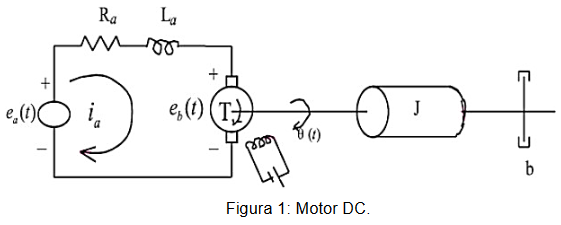
\includegraphics[width=0.4\textwidth]{media/motor-electromecanico}
		\caption{Esquema general de un motor DC}
		\label{fig:motor-electromecanico}
	\end{figure}
	
	Al aplicar la ley de tensiones de Kircchoff en el circuito de armadura, se tiene la siguiente relación:
	\begin{equation}
		R_ai(t) + L\frac{d}{dx} i(t) + K_b \frac{d}{dt} \theta (t) = e_a(t)
		\label{eq:malla-1}
	\end{equation}
	
	Esta relación eléctrica nos permite relacionar voltajes entre los diferentes componentes que integran al circuito de armadura del motor y la cual a su vez describen la parte eléctrica del sistema, siendo tales partes las siguientes y las que se considerarán para el modelo a construir en MATLAB. \\
	
	$R_a = 17 \Omega$ \\
	$L_a = 9.35*10^-3 H$ \\
	$K_e = 0.0436 \frac{Vs}{rad}$ \\
	$K_m = 0.0436 \frac{N-m}{A}$ \\
	
	Además en la ecuación \ref{eq:malla-1} se debe tener en cuenta la equivalencia para la constante contra electromotriz y la cual esta relacionada con la frecuencia angular mediante la siguiente expresión
	\begin{equation}
		e_b(t) = K_e\frac{d}{dt} \theta(t)
		\label{eq:contra-electromotriz}
	\end{equation}
	
	Obteniéndose de esta forma la ecuación \ref{eq:malla-1}, al analizar tal expresión se puede destacar que se cuenta con un termino en función de la frecuencia angular, sin embargo aun es necesario despejar la corriente en función del anterior parámetro, por ello es necesario utilizar la siguiente constante (par del motor) $K_m$ y los diagramas de cuerpo libre en la parte mecánica, obteniéndose las siguientes relaciones:
	
	\begin{align}
		T &= \ddot{\theta}J + \dot{\theta}b \label{eq:diagrama-cuerpo-libre}\\ 
		T &= K_mi(t) \label{eq:constate-torque}
	\end{align}
	
	Al reemplazar la ecuación \ref{eq:diagrama-cuerpo-libre} y \ref{eq:constate-torque} y despejar la corriente, se tiene la siguiente expresión analítica:
	
	\begin{equation}
		i(t) = \frac{ \ddot{\theta}J + \dot{\theta}b }{ K_m }
		\label{eq:corriente-torque}
	\end{equation}
	
	Una vez obtenidas todas estas relaciones será necesario aplicar la transformada de Laplace $\mathcal{L}\{f(t)\}$ para transformar cada ecuación al dominio de la frecuencia y obtener una relación entre la $\omega(s)$ (frecuencia angular) y $E_a(S)$ la cual es la función de transferencia deseada, obteniendo.
	
	\begin{align}
		E_a(S) &= I(S)\{R_a + LS\} + K_eS\theta(S) \label{eq:malla-1-laplace} \\
		T(S) &= \theta(S)JS^2 + \theta(S)bS \label{eq:torque-laplace} \\
		I(S) &= \frac{\theta(S)JS^2 + \theta(S)bS}{K_m} \label{eq:corriente-laplace}
	\end{align}
	
	Finalmente al reemplazar la ecuación \ref{eq:corriente-laplace} en \ref{eq:malla-1-laplace} se tendrá la siguiente expresión resultante de la cual será posible obtener la función de transferencia, la cual se representa de la siguiente forma:
	
	\begin{equation}
		\frac{\omega(S)}{E_a(S)} = \frac{K_m}{JLS^2 + (JR_a + Lb)S + (bR_a + K_eK_m)}
		\label{eq:ft-motor}
	\end{equation}
	
	De esta expresión final 
	
	\bibliographystyle{IEEEtran}
	\bibliography{biblio}
\end{document}
